% Chapter 10, Section 5

\section{Sequence-to-Sequence Models \difficultyInline{intermediate}}
\label{sec:seq2seq}

\subsection*{Intuition}

Encoder–decoder models compress a source sequence into a representation and then generate a target sequence step-by-step. Attention augments this by letting the decoder look back at encoder states as needed, creating a dynamic context per output token \cite{Cho2014,Bahdanau2014}.

\subsection*{Historical Context}

Early seq2seq relied on fixed context vectors, which degraded on long inputs. Content-based attention \cite{Bahdanau2014} lifted this bottleneck and paved the way toward Transformer architectures \cite{Vaswani2017}.

% Index and glossary
\index{sequence-to-sequence}
\glsadd{attention-mechanism}

\subsection{Encoder-Decoder Architecture}

For sequence transduction tasks like machine translation \cite{Cho2014,Bahdanau2014}:

\textbf{Encoder:} Processes input sequence into representation (fixed or per-step states)
\begin{equation}
\vect{c} = f(\vect{x}_1, \vect{x}_2, \ldots, \vect{x}_T)
\end{equation}

\textbf{Decoder:} Generates output sequence from representation
\paragraph{Visual aid.} A minimal encoder–decoder with context vector.
\begin{figure}[h]
    \centering
    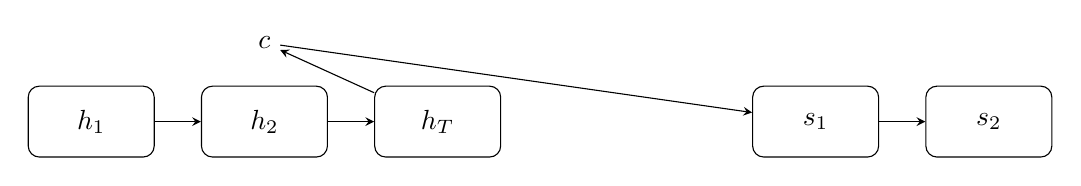
\begin{tikzpicture}[>=stealth, node distance=2.2cm]
        \tikzstyle{enc}=[draw, rounded corners, minimum width=1.6cm, minimum height=0.9cm]
        \tikzstyle{dec}=[draw, rounded corners, minimum width=1.6cm, minimum height=0.9cm]
        \node[enc] (e1) {$\vect{h}_1$};
        \node[enc, right of=e1] (e2) {$\vect{h}_2$};
        \node[enc, right of=e2] (eT) {$\vect{h}_T$};
        \node[above of=e2, yshift=-1.2cm] (c) {$\vect{c}$};
        \draw[->] (e1) -- (e2);
        \draw[->] (e2) -- (eT);
        \draw[->] (eT) -- (c);
        \node[dec, right of=eT, xshift=2.6cm] (d1) {$\vect{s}_1$};
        \node[dec, right of=d1] (d2) {$\vect{s}_2$};
        \draw[->] (c) -- (d1);
        \draw[->] (d1) -- (d2);
    \end{tikzpicture}
    \caption{Encoder–decoder with a fixed context vector $\vect{c}$. Attention replaces $\vect{c}$ with step-dependent $\vect{c}_t$.}
\end{figure}

\begin{equation}
\vect{y}_t = g(\vect{y}_{t-1}, \vect{c}, \vect{s}_{t-1})
\end{equation}

\subsection{Attention Mechanism}

Standard seq2seq compresses entire input into fixed vector $\vect{c}$, causing information bottleneck.

\textbf{Attention} allows the decoder to focus on relevant input parts by computing a content-based weighted average of encoder states \cite{Bahdanau2014}. At each decoding step $t$:

\begin{align}
e_{ti} &= a(\vect{s}_{t-1}, \vect{h}_i) \quad \text{(alignment scores)} \\
\alpha_{ti} &= \frac{\exp(e_{ti})}{\sum_j \exp(e_{tj})} \quad \text{(attention weights)} \\
\vect{c}_t &= \sum_i \alpha_{ti} \vect{h}_i \quad \text{(context vector)}
\end{align}
Common scoring functions $a(\cdot)$ include additive (Bahdanau) attention using a small MLP, and multiplicative/dot-product attention which is parameter-efficient and forms the basis for scaled dot-product attention in Transformers \cite{Vaswani2017}. Attention weights $\alpha_{ti}$ are interpretable as soft alignments between target position $t$ and source position $i$ (see \cite{WebAttentionWikipedia}). For a broader overview, consult standard references \cite{WebDLBRNN,D2LChapterAttention}.

\paragraph{Training and inference.} Attention is trained end-to-end with the seq2seq objective. During inference, attention enables the model to retrieve the most relevant encoder features for each generated token, improving long-input performance and handling reordering. Variants include multi-head attention, local/monotonic attention for streaming, and coverage terms to reduce repetition.

Benefits:
\begin{itemize}
    \item Dynamic context for each output
    \item Better for long sequences
    \item Interpretable (visualize attention weights)
\end{itemize}

\subsection{Applications}

\begin{itemize}
    \item Machine translation (NMT)
    \item Text summarization (extractive and abstractive)
    \item Question answering and dialogue systems
    \item Image captioning (CNN/ViT encoder, RNN/Transformer decoder)
    \item Speech recognition and speech translation
    \item OCR and handwriting recognition
    \item Code generation and program repair
\end{itemize}

